\section{Progressive-Adaptive Music Generator for Videogames}

The last approach hence of adaptive and generative music
was published in 2023 by Alvaro Eduardo Lopez Duarte \cite{lopez2023progressive}.
It was developed to generate music for 
video games in real-time \cite{lopez2023progressive}.
The system of Lopez can be categorized in various categories of generative music \cite{lopez2023progressive}. It takes on the role of composing and arranging by creating new pieces of music and recombining existing melody lines and chords \cite{lopez2023progressive}. It also adapts the interpretation by changing parameters \cite{lopez2023progressive}. PAMG manages both the horizontal (temporal sequences) and vertical (simultaneous musical events) directions in the music \cite{lopez2023progressive}. It works at different levels of granularity such as phrases, bars, beats, notes and chords and uses a coarse grid as the minimum event duration, with the exception of arpeggios, ratchets and staccato events \cite{lopez2023progressive}.

In gameplay context, the music of the author's PAMG is non-
diegetic, which means it is not generated within the game 
world,
instead it belongs to the narrative representation of the
game \cite{lopez2023progressive}. The music within the game is ambient, that means it is
not tied to a specific source, and adaptive, as it changes 
based on game variables \cite{lopez2023progressive}. However, PAMG can also make changes
autonomously \cite{lopez2023progressive}.

The system consists of several agents, which are able to
adapt and create melodies, harmonies and rhythms 
\cite{lopez2023progressive}. The main components of 
the system are the Melody Agent, the Harmony Agent, the 
Percussion Agent and the Orchestrator Agent
\cite{lopez2023progressive}. The Melody Agent creates
and manages melodies, the Harmony Agent takes care of
the harmonies and chords, the Percussion Agent takes care
of rhytmic Elements and the Orchestrator Agent assigns
instruments families and makes real-time decisions on the
instrument usage \cite{lopez2023progressive}. Next to those
agents, a Multi-Parameter Preset Interpolator and Controller
(MPIC) enables control and interpolation between different 
presets, allowing smooth transitions between different 
musical settings \cite{lopez2023progressive}. The descripted
algorithm process can be seen in \Cref{fig:pamg_algorithm}

\begin{figure}[h]
    \centering
    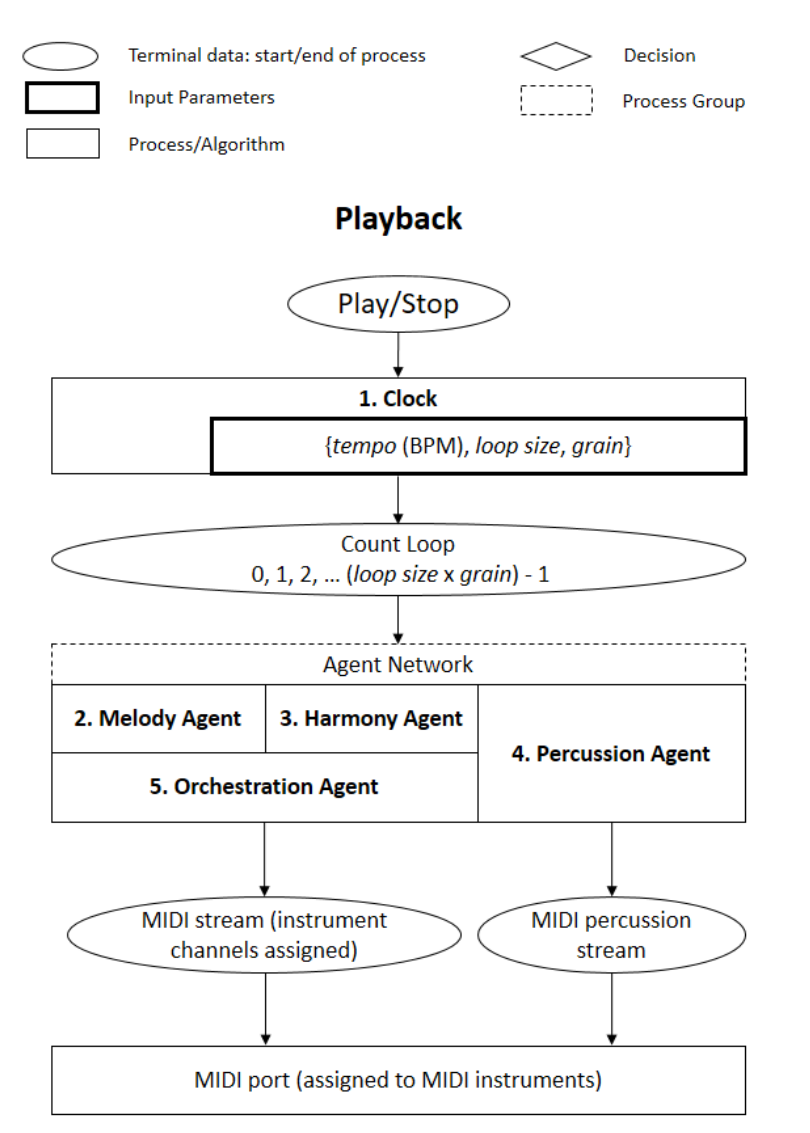
\includegraphics[width=\linewidth,height=10cm]{images/pamg_algorithm.png}
    \caption{Algorithm / architecture of PAMG \cite{lopez2023progressive}}
    \label{fig:pamg_algorithm}
\end{figure}


\subsubsection{Melody Agent}

The Melody Agent is responsible for generating melodies as outlined in previous sections \cite{lopez2023progressive}. Initially, the Melody Agent engages in rhythm generation by producing a list of onsets based on the beat, which is then manipulated to create syncopation. This process yields two lists: the Moved List and the Beat List \cite{lopez2023progressive}. Subsequently, the onsets are subject to stochastic modifications, either added or removed randomly from these lists \cite{lopez2023progressive}. The duration of each onset is then determined, classified as either staccato or legato \cite{lopez2023progressive}.

Following the completion of rhythm generation, the next step is velocity generation \cite{lopez2023progressive}. This involves employing a stochastic sequence to determine the MIDI velocity, or amplitude, for each onset, ultimately producing a MIDI velocity value for every onset \cite{lopez2023progressive}.

Pitch generation occurs after velocity determination \cite{lopez2023progressive}. This phase comprises three sub-processes: note stream generation, transposition, and harmony filtering \cite{lopez2023progressive}. The algorithm incorporates both "drunk" and "drunk-contour" modes for pitch generation, with each mode producing a pitch value that is subsequently adjusted through the transposition algorithm to refine the pitch \cite{lopez2023progressive}. A harmony filter is then applied to harmonize the pitch value \cite{lopez2023progressive}.

Once pitch generation is complete, the melody is developed through temporal transposition \cite{lopez2023progressive}. Subsequently, melody modification involves changing the transposition based on an analysis of previous pitches and generating new transposition values \cite{lopez2023progressive}. Additionally, phrase changes are implemented, altering rhythmic patterns according to harmonic structures \cite{lopez2023progressive}. These modifications are integrated into the MIDI event construction, resulting in a MIDI event stream that is forwarded to the Orchestration Agent \cite{lopez2023progressive}.

\subsubsection{Harmony Agent}

The Harmony Agent commences with the generation of harmony rhythm \cite{lopez2023progressive}. This involves operating an accent/beat follower to produce an interpolated list of rhythmic accents derived from the Moved List and Beat List \cite{lopez2023progressive}. A seeded random generator is used to introduce syncopation or adherence to beats \cite{lopez2023progressive}. Following this, the generated onsets are adjusted by adding or subtracting onsets based on harmony parameters \cite{lopez2023progressive}. A binary sequence for staccato/legato is then applied to determine the duration of each onset \cite{lopez2023progressive}.

After rhythm generation, the Harmony Agent progresses to velocity generation \cite{lopez2023progressive}. This step involves creating MIDI velocity values for chord onsets or arpeggio pitches, with a focus on onsets from the Moved List \cite{lopez2023progressive}.

The subsequent process is harmony sequence generation \cite{lopez2023progressive}. The module selects chord changes within a loop, ensuring that certain transitions are avoided at the beginning and end to facilitate longer resolutions \cite{lopez2023progressive}. It manages chord pools and their progression, determining the available chords and their sequence based on complexity \cite{lopez2023progressive}. Using a chord dictionary, pitch-class lists for chords are retrieved and adjusted for dissonance if required \cite{lopez2023progressive}. The chord builder then constructs pitch lists for playback, organizing intervals to emulate orchestration, while the arpeggiator generates arpeggio patterns based on orchestration settings and other parameters \cite{lopez2023progressive}.

Following the completion of harmony sequence generation, the harmony change algorithm prepares and implements changes to register and onset parameters, utilizing a random generator with constraints to prevent frequent modifications \cite{lopez2023progressive}. MIDI event construction then integrates all calculated outputs to produce a MIDI stream, which is forwarded to the Orchestration Agent \cite{lopez2023progressive}.


\subsubsection{Percussion Agent}

The Percussion Agent is responsible for generating rhythms for percussion instruments using various algorithms \cite{lopez2023progressive}. The Accent/Beat Follower interpolates syncopations for all percussion instruments based on the Moved List and Beat List \cite{lopez2023progressive}. The Additive and Subtractive Filling algorithm then allocates these onsets to different percussion instruments, such as kick/snare, toms, and cymbals, allowing for customizable patterns and offsets \cite{lopez2023progressive}.

Velocity generation determines the velocity parameter to set accents and produce MIDI velocity values \cite{lopez2023progressive}. The ratchet mechanism randomly selects the occurrence and type of ratchet (e.g., 64th, 32nd) for all instruments except the kick drum, calculating the corresponding velocity values \cite{lopez2023progressive}.

The percussion change function adjusts percussion parameters based on current chords to create variations. A random generator is used to determine changes that support the phrasing \cite{lopez2023progressive}.

In MIDI event construction, the Percussion Agent manages the pitch range of each instrument in MIDI pitch values and generates real-time MIDI events based on velocity, pitch, and a constant duration of 300 ms \cite{lopez2023progressive}. Non-zero values from the rhythm onset collection are used to trigger the generation of onsets, which are then formed into MIDI events \cite{lopez2023progressive}.

\subsubsection{Orcestration Agent}

The Orchestration Agent uses a random generator to manage the instrument families of the Melody/Harmony agents \cite{lopez2023progressive}. It adds or removes instruments for each agent by adjusting the Orch +/- parameters and distributes the instrument families to the Harmony Agent stream voices based on the Harmony Agent velocity (intensity when overlapping), voices and range parameters \cite{lopez2023progressive}. The instrument change occurs after two phrases without orchestration changes \cite{lopez2023progressive}. It sets the range for the Melody Agent's instrument voices using the Orch Range parameter and the Pitch Class List \cite{lopez2023progressive}. Flags are sent to the arpeggiator algorithm for solo brass and solo piano and receive arpeggiator on/off signals \cite{lopez2023progressive}. The instrument family range is managed via the pitch frame in MIDI pitch values (a non-real-time parameter) \cite{lopez2023progressive}. Finally, the agent sends the final MIDI events to the specified MIDI channels and ports \cite{lopez2023progressive}.